\chapter{Resultados e produtos obtidos}

\section{Implementação concorrentes dos Métodos Runge-Kutta, Nearest Neighbour e Interpolação Linear}
  \subsection{Protótipo básico}
  O protótipo básico foi uma prova de conceito bem sucedida para a implementação do método implementação em si e suas limitações, bem como para o uso das linguagens CUDA e OpenCL para este fim.
  
  Sua compilação é bastante simples através do comando \textit{make}. Sem nenhum argumento ele compilará a versão em \textit{C++} por padrão. Com os argumentos \textit{cuda} ou \textit{opencl} serão compiladas suas respectivas versões.
  
  \begin{figure}[!h]
    \begin{center}
      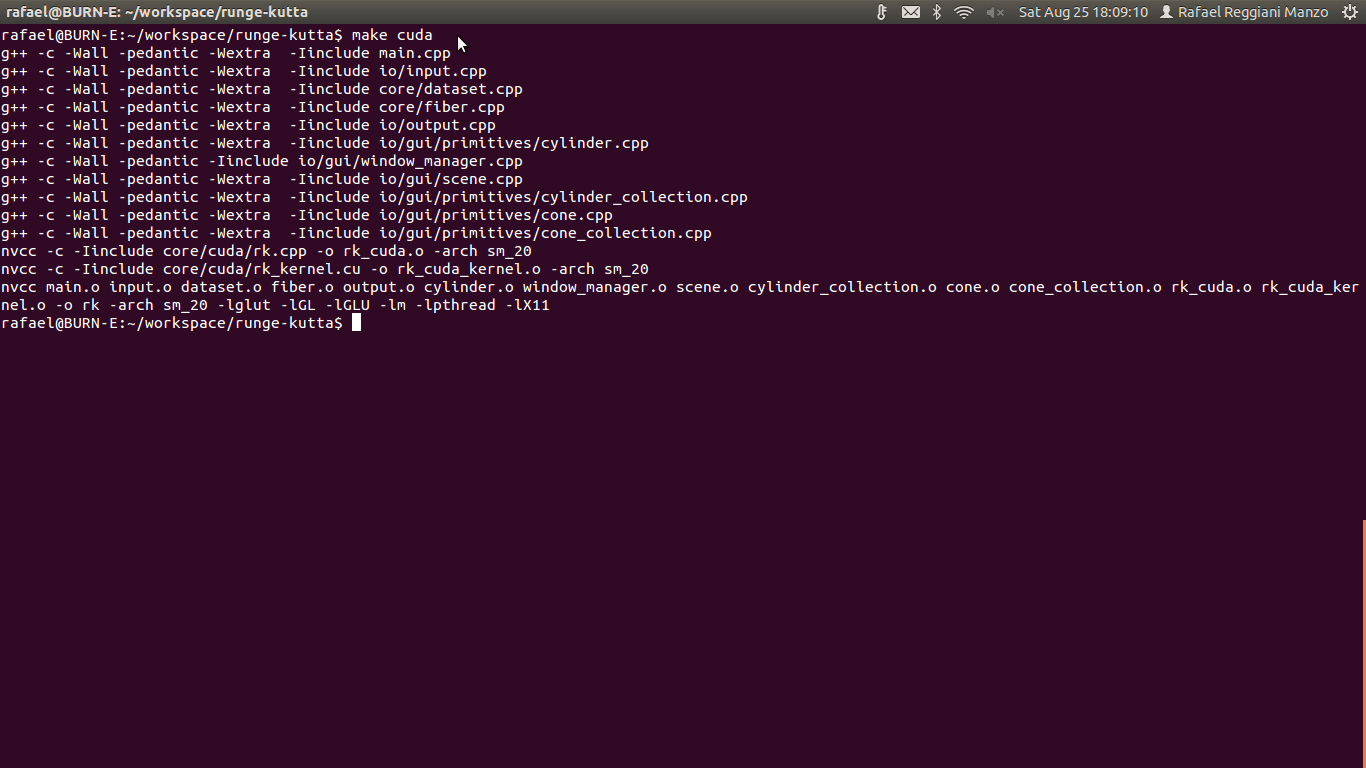
\includegraphics[width=140mm, height=80mm]{images/compilacao.png}
      \label{fig:}
      \caption{Compilação da versão CUDA}
    \end{center}
  \end{figure}
  
  \newpage  
  Sua interface é bastante básica, mas permite rotacionar o campo e a fibra, translada-lo, aproximá-lo ou afasta-lo tudo através de teclas. Além disso, é possível escolher quais informações são exibidas. Ou seja, é possível escolher entre exibir ou ocultar o campo vetorial, as fibras resultantes do RK2 ou as fibras resultantes do RK4.
  
  A única limitação encontrada para esta implementação é lidar com a inderteminação que existe no campo vetorial na região de intersecção de duas fibras. Esta indeterminação faz com que o método possa seguir qualquer uma das fibras na intersecção quando chega a esta região.
  
  \begin{figure}[!h]
    \begin{center}
      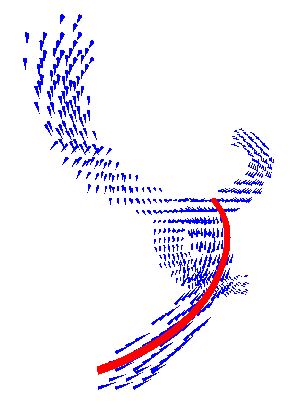
\includegraphics[width=140mm, height=80mm]{images/fibraecampo.png}
      \label{fig:}
      \caption{Campo 32x32x32 com duas hélices. Ao chegar na intersecção, a fibra se desvia para um fora do campo e o método entende que terminou de propaga-la devido à baixa intensidade dos vetores.}
    \end{center}
  \end{figure}
  
  \newpage
  \subsection{Protótipo utilizando a VTK}
\section{Integração com o MedSquare}
